% 0. Preamble: -----------------------------------------------------{{{
% 0.1 Document Class Setup: ----------------------------------------{{{

\documentclass[12pt]{article}

%}}}
% 0.2 Packages + Libraries: ----------------------------------------{{{

\usepackage{amsmath,amsfonts,mathtools,graphicx,amssymb,dirtytalk}
\usepackage[margin=0.21in]{geometry}
\usepackage[]{microtype}
\graphicspath{{./3-img/}}
% using tikz, for Venn diagrams in this case
\usepackage{tikz}
% using tikz commands (must come after \usepackage{tikz})
% http://users.ju.edu/hduong/math220/venn_diagrams.pdf
\usetikzlibrary{shapes, backgrounds}

%}}}
% 0.3 Commands: ----------------------------------------------------{{{

% binomial exponent
\newcommand{\negativeBinomial}[3][2]{(#2- #3)^{#1}}
% large math
\newcommand*{\largeMath}[1]{\mbox{\Large$#1$}}
% huge math
\newcommand*{\hugeMath}[1]{\mbox{\huge$#1$}}

%}}}
%}}}
\begin{document}
% Section: Section Template: ---------------------------------------{{{
\section*{Section Template: This is a template for a section}
  % Setup: Template: -----------------------------------------------{{{

  \paragraph{Add setup content here, datasets, info, etc.}
  \begin{align*}
    X = \{a, b, c\} && \text{AND} &&
    Y = \{1, 2, 3\}
  \end{align*}

  %}}}
  % Subsection: Template: ------------------------------------------{{{

  \subsection{Subsection Template}
  \paragraph{Description:} This is the template for a subsection.
  \paragraph{Quote:} \say{Here is an example quote}
  \paragraph{Definition:} A definition could be added here.
  \paragraph{Visualization:} $\LaTeX, \TeX$, Tikz, graphicx, or Python, matplotlib, etc.

  \begin{align}
    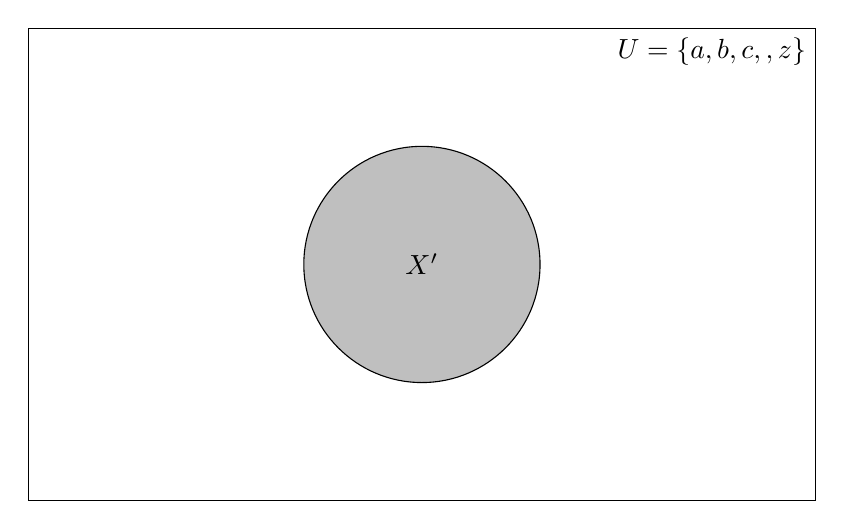
\begin{tikzpicture}
      \draw (-5,-3) rectangle (5,3) node[below left]{$U= \{a, b, c, \ldot, z\}$};
      \fill[lightgray] (0,0) circle (1.5cm) node {$X'$};
      \draw (0,0) circle (1.5cm) node {$X'$};
    \end{tikzpicture} && % chktex 31
    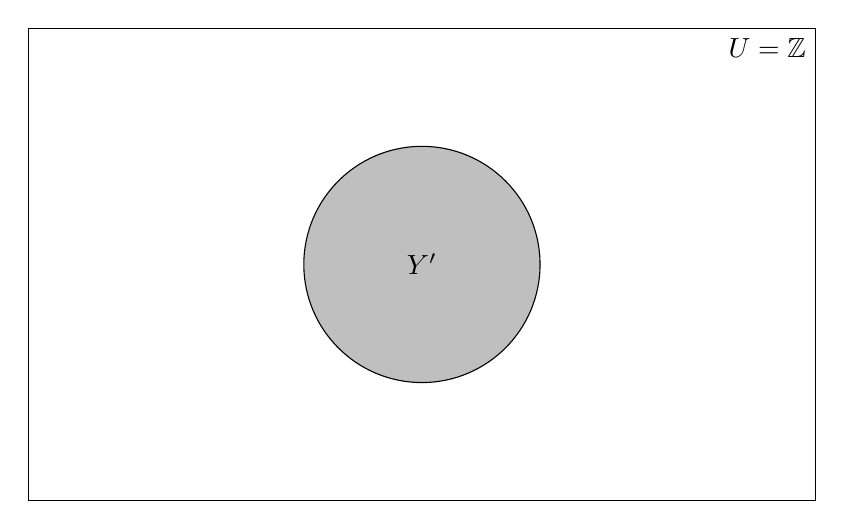
\begin{tikzpicture}
      \draw (-5,-3) rectangle (5,3) node[below left]{$U=\mathbb{Z}$};
      \fill[lightgray] (0,0) circle (1.5cm) node {$Y'$};
      \draw (0,0) circle (1.5cm)  node {$Y'$};
    \end{tikzpicture}
  \end{align}

  \paragraph{Solution:} Maybe add solutions here..
  \paragraph{Intuition:} Or findings, explanations, etc.

  \begin{align*}
    X' = \{d, e, f,\ldots z\} && Y' \neq \{1, 2, 3\}
  \end{align*}

  %}}}
%}}}
\end{document}
